
\section{Comunicação com o robô}

Como o plano original era usar o microcontrolador STM32,
a comunicação mais simples e direta de implementar seria uma comunicação serial com um módulo Bluetooth.
Foi considerando comunicação via rádio, porém exigiria um investimento na aquisição de um controle RC.
Uma comunicação Bluetooth exige apenas a integração de um aplicação Android para enviar dados via Bluetooth.

\subsection{Módulo HC-05 vs ESP-WROOM-32}

Na seção \ref{microcontrolador_ide} foi discutido a mudança do microcontrolador STM32 para o ESP32.
e como o uso do módulo HC-05 exigia um nível de atenção maior ao escrever um novo programa no STM32.
A alteração para o ESP32, com o chip ESP-WROOM-32 (com Bluetooth e Wi.fi integrado) não exigiu muitas alterações no projeto.
Pois, o componente Bluetooth é controlado como se fosse uma comunicação serial.

\noindent
\begin{minipage}[t]{0.48\textwidth}
\captionsetup{labelformat=empty}
\begin{lstlisting}[
    language=C,
    caption={Comunicação entre STM32 e HC-05}
]
#include <HardwareSerial.h>
#include <libmaple/usart.h>

void setup() {
    pinMode(RX_STM_PIN, INPUT);
    pinMode(TX_STM_PIN, OUTPUT);
    Serial3.begin(9600);
    Serial.begin(9600);
};
\end{lstlisting}
\end{minipage}
\hfill
\begin{minipage}[t]{0.48\textwidth}
\captionsetup{labelformat=empty}
\begin{lstlisting}[
    language=C,
    caption={Comunicação com Bluetooth integrado}
]
#include "BluetoothSerial.h"

BluetoothSerial SerialBT;

void setup() {
    SerialBT.begin("deviceName");
    Serial.begin(115200);
};
\end{lstlisting}
\end{minipage}

\subsection{Aplicativo Android}

\subsubsection{Controle de direção}

O aplicativo Arduino Bluetooth Controller possui uma opção em que o aplicativo envia uma
'string' representando as cores RGB em 'int8'.
por exemplo,  vermelho seria '255000000' (r=255, g=0, b=0).
E a interface é o modelo de cor HSV em 2 dimensões de ponta cabeça,
\autoref{arduino_bluetooth_controller_hsl_model}.


\begin{figure}[htb]
	\centering
	\caption{Tela de controle RGB do aplicativo Arduino Bluetooth Controller}
	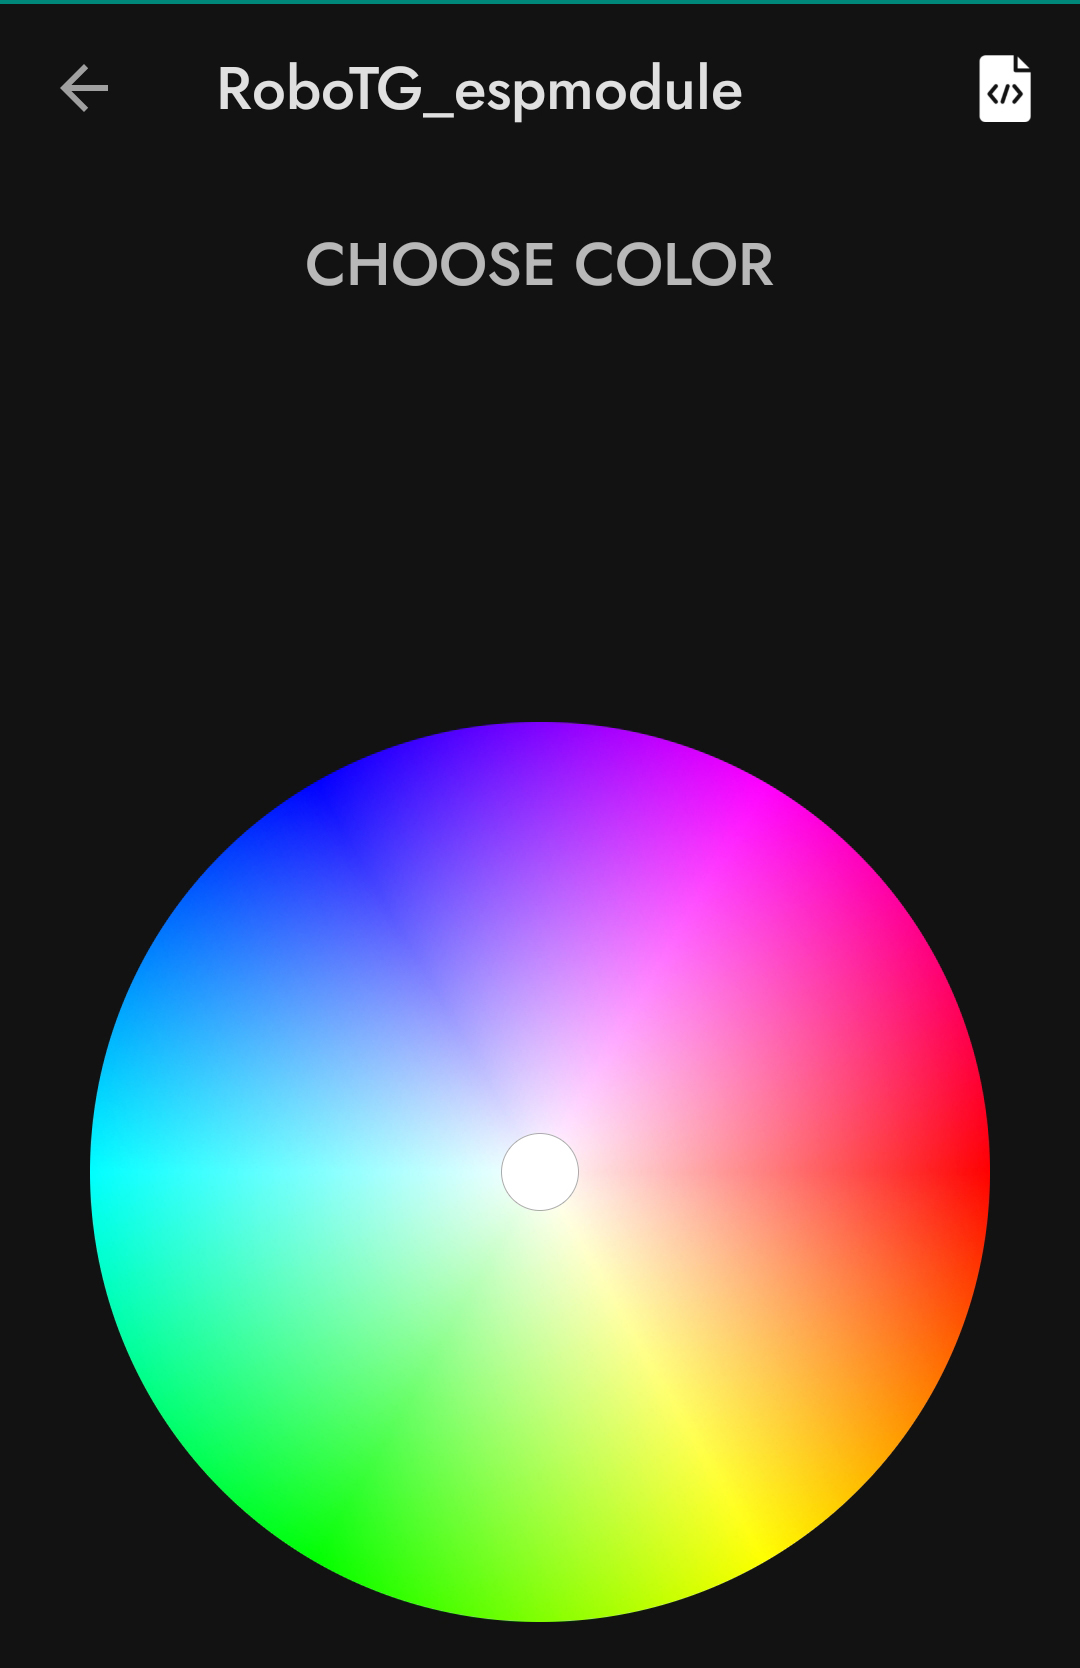
\includegraphics[width=0.40\textwidth]{figures/andriod_bluetooth_controller_hsl_model}
    \caption*{FONTE: Própria}
	\label{arduino_bluetooth_controller_hsl_model}
\end{figure}

No modelo HSV,  a \autoref{rbg_hsl_hsv}, 'H' significa "hue" ou matiz, e é 
um valor do angulo no modelo HSV, 'S' significa 'saturação' e corresponde a um valor de raio,
por último, 'V' é valor, que corresponde a uma terceira dimensão, 
que não aparece no modelo bidimensional disponível no aplicativo.
Exitem outros dois modelos parecidos que usam a mesma representação cilíndrica, 
HSL, e HSB, que possuem uma lógica semelhando ao HSV.


\begin{figure}[htb]
	\centering
	\caption{Modelos RGB, HSL e HSV}
	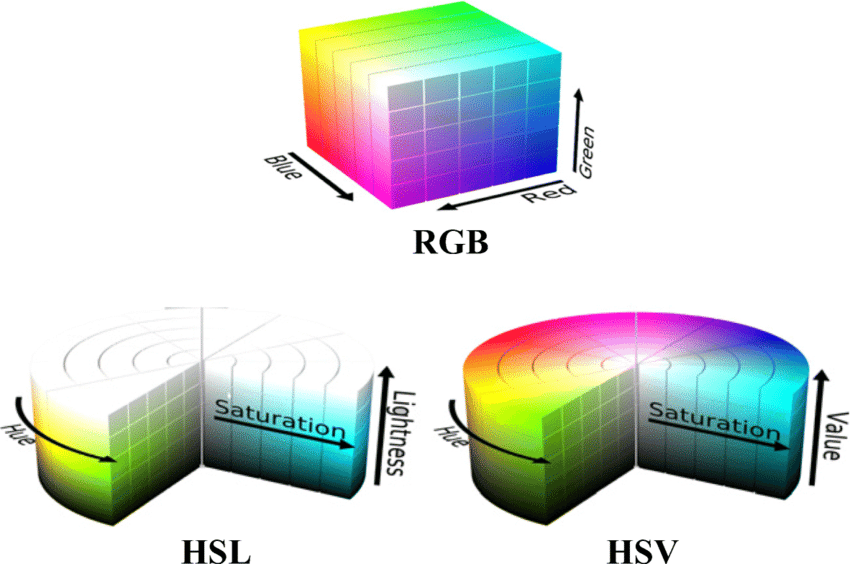
\includegraphics[width=0.6\textwidth]{figures/RBG_HSL_HSV}
	\caption*{
        FONTE: Saturation-aware human attention region of interest algorithm for
        efficient video compression - N'guessan, Sylvia and Ling, Nam \cite{rbg_hsl_hsv}
    }
	\label{rbg_hsl_hsv}
\end{figure}

\begin{figure}[htb]
	\centering
	\caption{Modelo HSV bidimensional \cite{hsv_model}}
	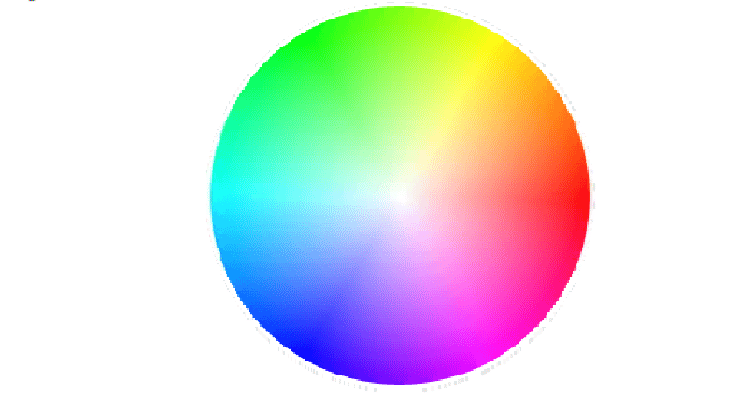
\includegraphics[width=0.8\textwidth]{figures/HSV}
	\caption*{FONTE: An adaptation of the GAIA visualization method for cartography - Lidouh, Karim and De Smet, Yves and Zimanyi, Esteban \cite{hsv_model}}
\end{figure}


O aplicativo retorna os valores em RGB, então usando um algorítimo
que converte RGB para HSV e invertendo o eixo Y
é possível ter os valores de angulo e módulo de um vetor velocidade.
A \autoref{hsv_exemplo_1} possue os valores RBG enviados pelo aplicativo
e a posição em que o cursor do aplicativo esta,
Esses valors, quando aplicados no algorítimo de conversão de RGB para HSV, geram os resultados na \autoref{HSV_resultado}
Facilmente podemos extrair informações de direção e magnitude que podem ser usados para controlar o robô.
Como mencionado anteriormente, o modelo HSV esta invertido no eixo Y,
então para obter o angulo representado pelo aplicativo, basta de 360 o subtrair o valor encontrado.

\begin{figure}[htb]
	\centering
	\caption{Aplicativo Android - Valores RGB e posição}
	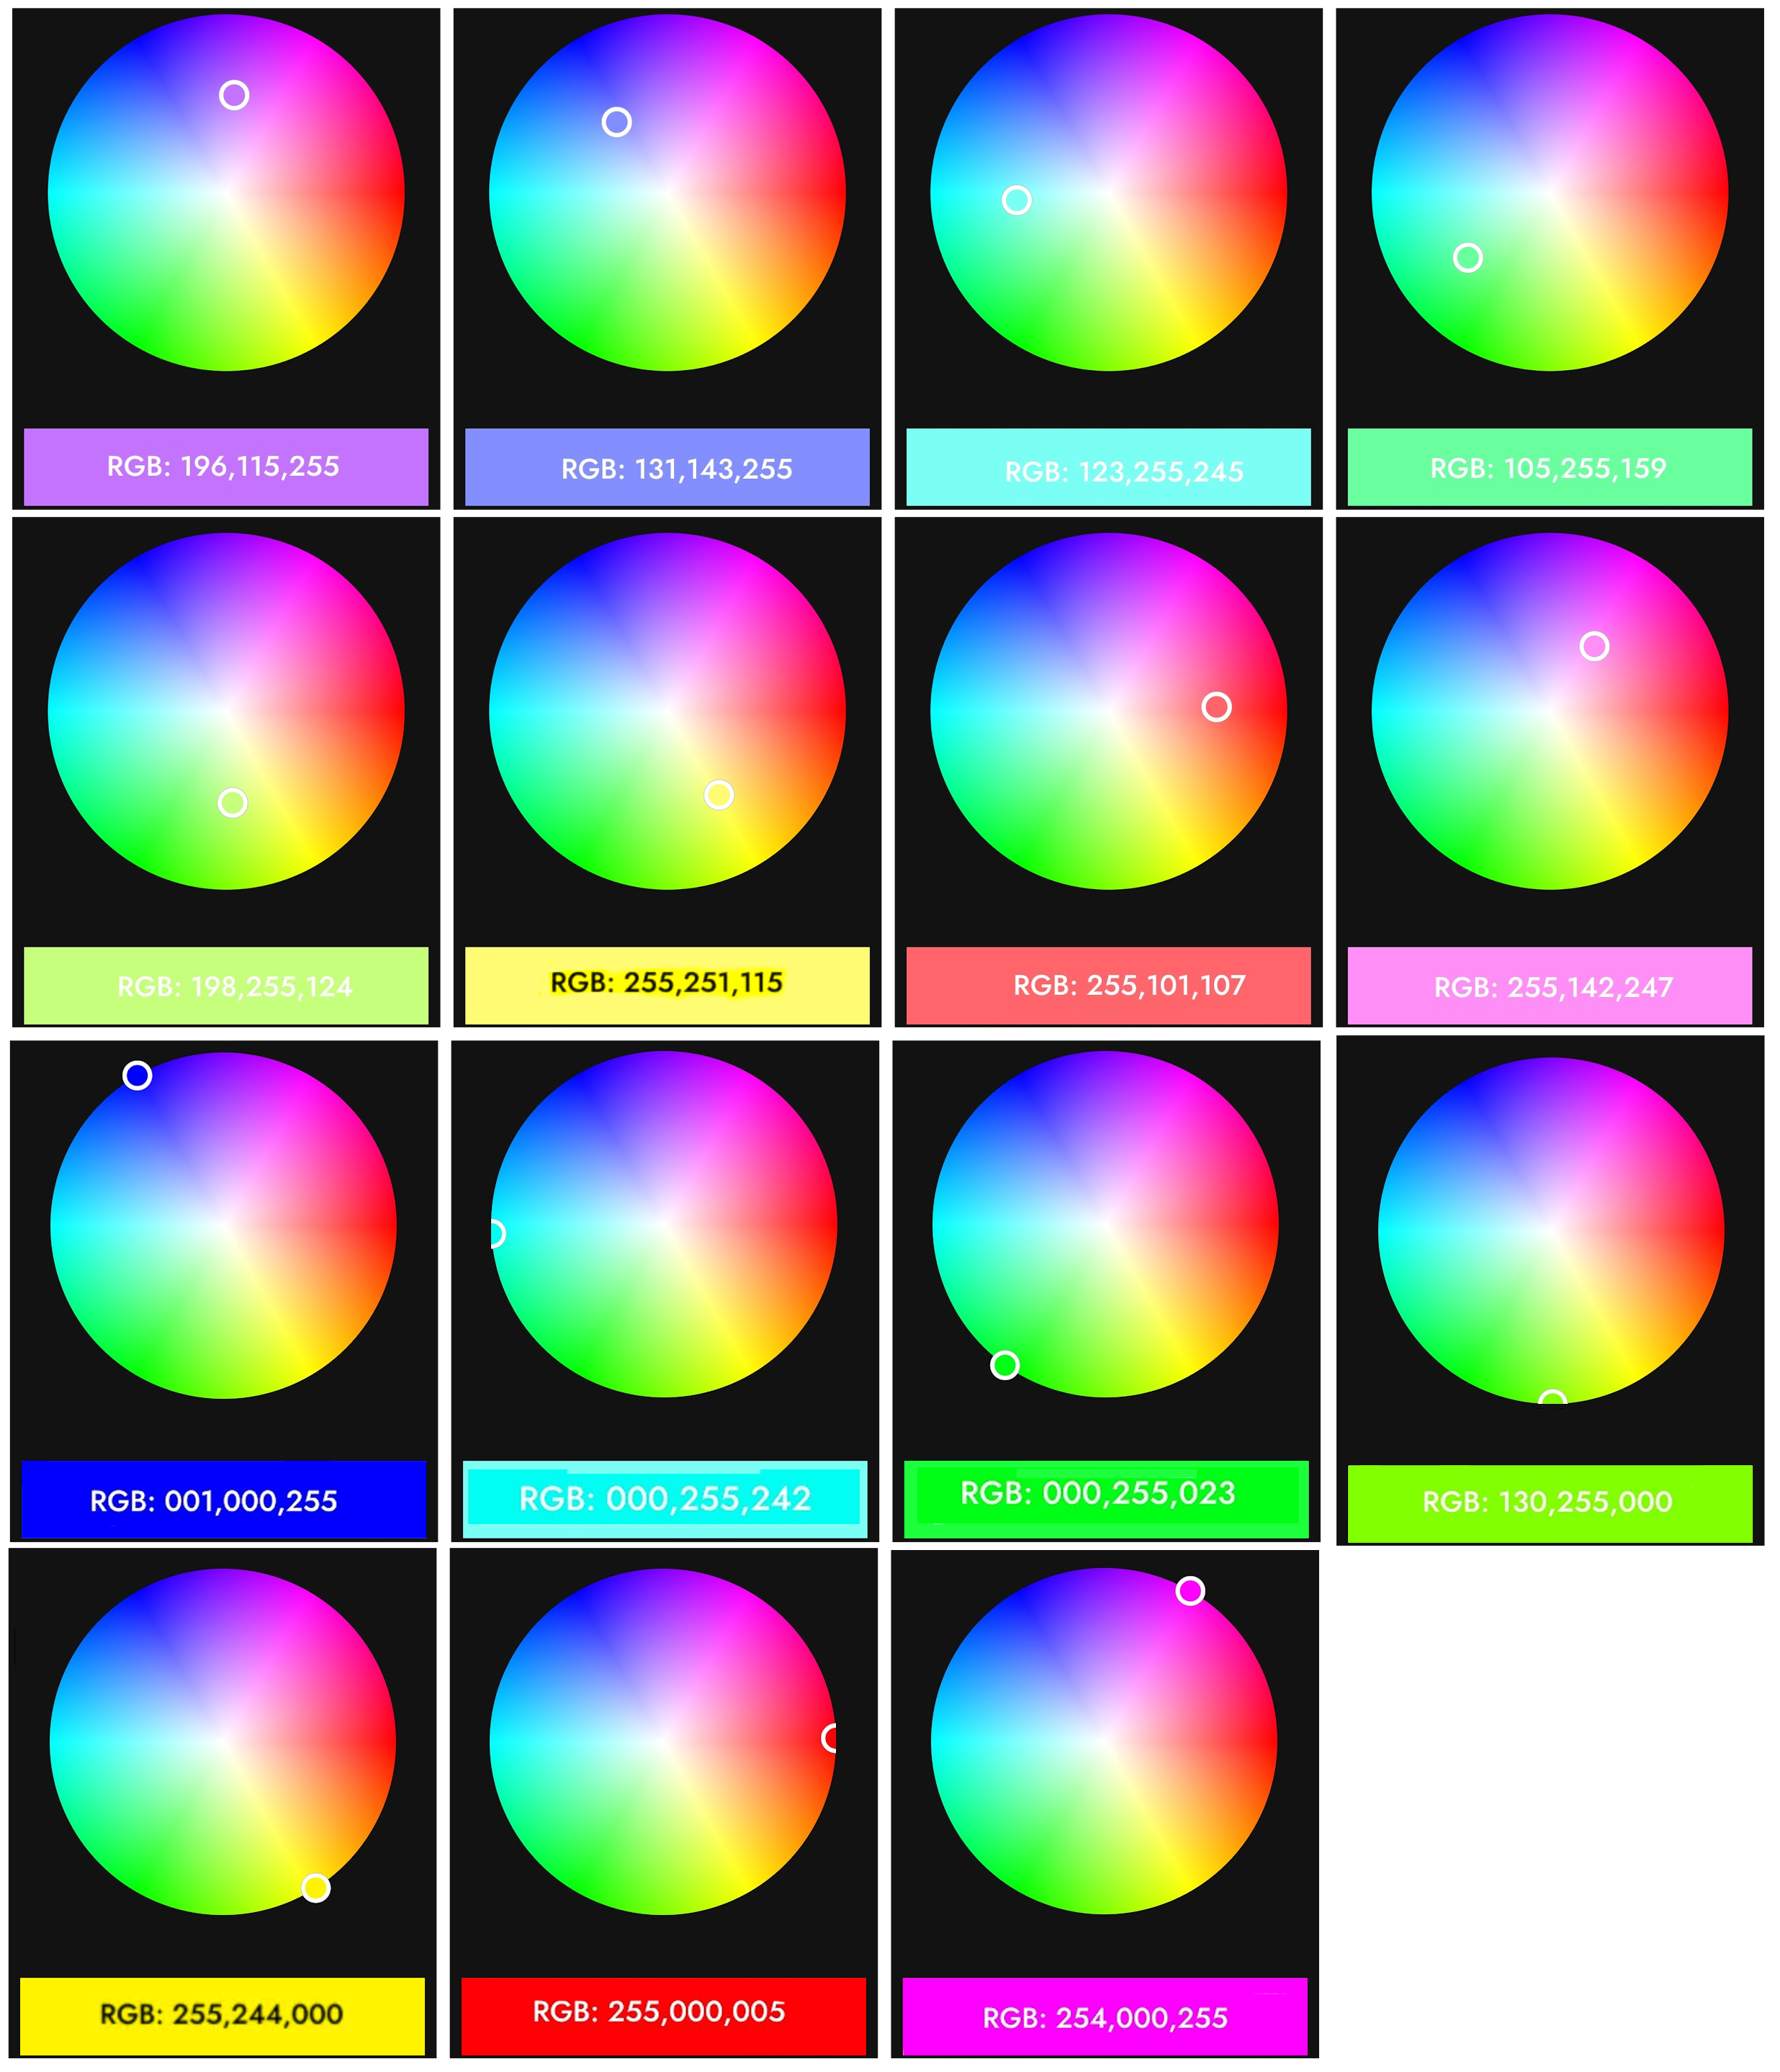
\includegraphics[width=1.0\textwidth]{figures/example_1_arduino_color}
	\caption*{FONTE: Própria}
	\label{hsv_exemplo_1}
\end{figure}


\begin{table}[ht]
	\centering
	\caption{\label{HSV_resultado}Resultado do algoritmo de conversão de RGB para HSV}
	\begin{tabular}{|c|c|c|c|}
        \hline
        \textbf{RGB} & \textbf{Ângulo $\theta$} & \textbf{Magniture} & \textbf{Correção de ângulo (360-$\theta$)} \\ \hline
        196, 115, 255 & 275\textdegree & 54,9\% & 85\textdegree \\ \hline
        131, 143, 255 & 234\textdegree & 48,63\% & 126\textdegree \\ \hline
        123, 255, 245 & 175\textdegree & 51,76\% & 185\textdegree \\ \hline
        105, 255, 159 & 142\textdegree & 58,82\% & 218\textdegree \\ \hline
        198, 255, 124 & 86\textdegree & 51,37\% & 274\textdegree \\ \hline
        255, 251, 115 & 58\textdegree & 54,9\% & 302\textdegree \\ \hline
        255, 101, 107 & 358\textdegree & 60,39\% & 2\textdegree \\ \hline
        255, 142, 247 & 304\textdegree & 44,31\% & 56\textdegree \\ \hline
        001, 000, 255 & 240\textdegree & 100,0\% & 120\textdegree \\ \hline
        000, 255, 242 & 177\textdegree & 100,0\% & 183\textdegree \\ \hline
        000, 255, 023 & 125\textdegree & 100,0\% & 235\textdegree \\ \hline
        130, 255, 000 & 89\textdegree & 100,0\% & 271\textdegree \\ \hline
        255, 244, 000 & 57\textdegree & 100,0\% & 303\textdegree \\ \hline
        255, 000, 005 & 359\textdegree & 100,0\% & 1\textdegree \\ \hline
        254, 000, 255 & 300\textdegree & 100,0\% & 60\textdegree \\ \hline
	\end{tabular}
\end{table}

O algoritmo de conversão de RGB para HSV transtrito em C, pode ser encontrado no apêndice \ref{rgb_to_hsv}.
É possível modificar o algoritmo para que o valor de magnitude seja mapeado em uma escala logaritma
para uma saida de velocidades maiores que zero de maineira mais suave,
e também é possível definir um diametro mínimo onde os valores
de magnitude seja sempre zero, dessa forma não é necessário muito
precisão do usuário para chegar em valores de zero.

\subsubsection{Demais controles}

Para demais ações e comandos para serem enviados para o microcontrolador
o aplicativo Serial Bluetooth Terminal permite enviar textos via terminal,
e atrelar textos predeterminados em botões de ação.

\begin{figure}[htb]
	\centering
	\caption{Tela do aplicativoSerial Bluetooth Terminal}
	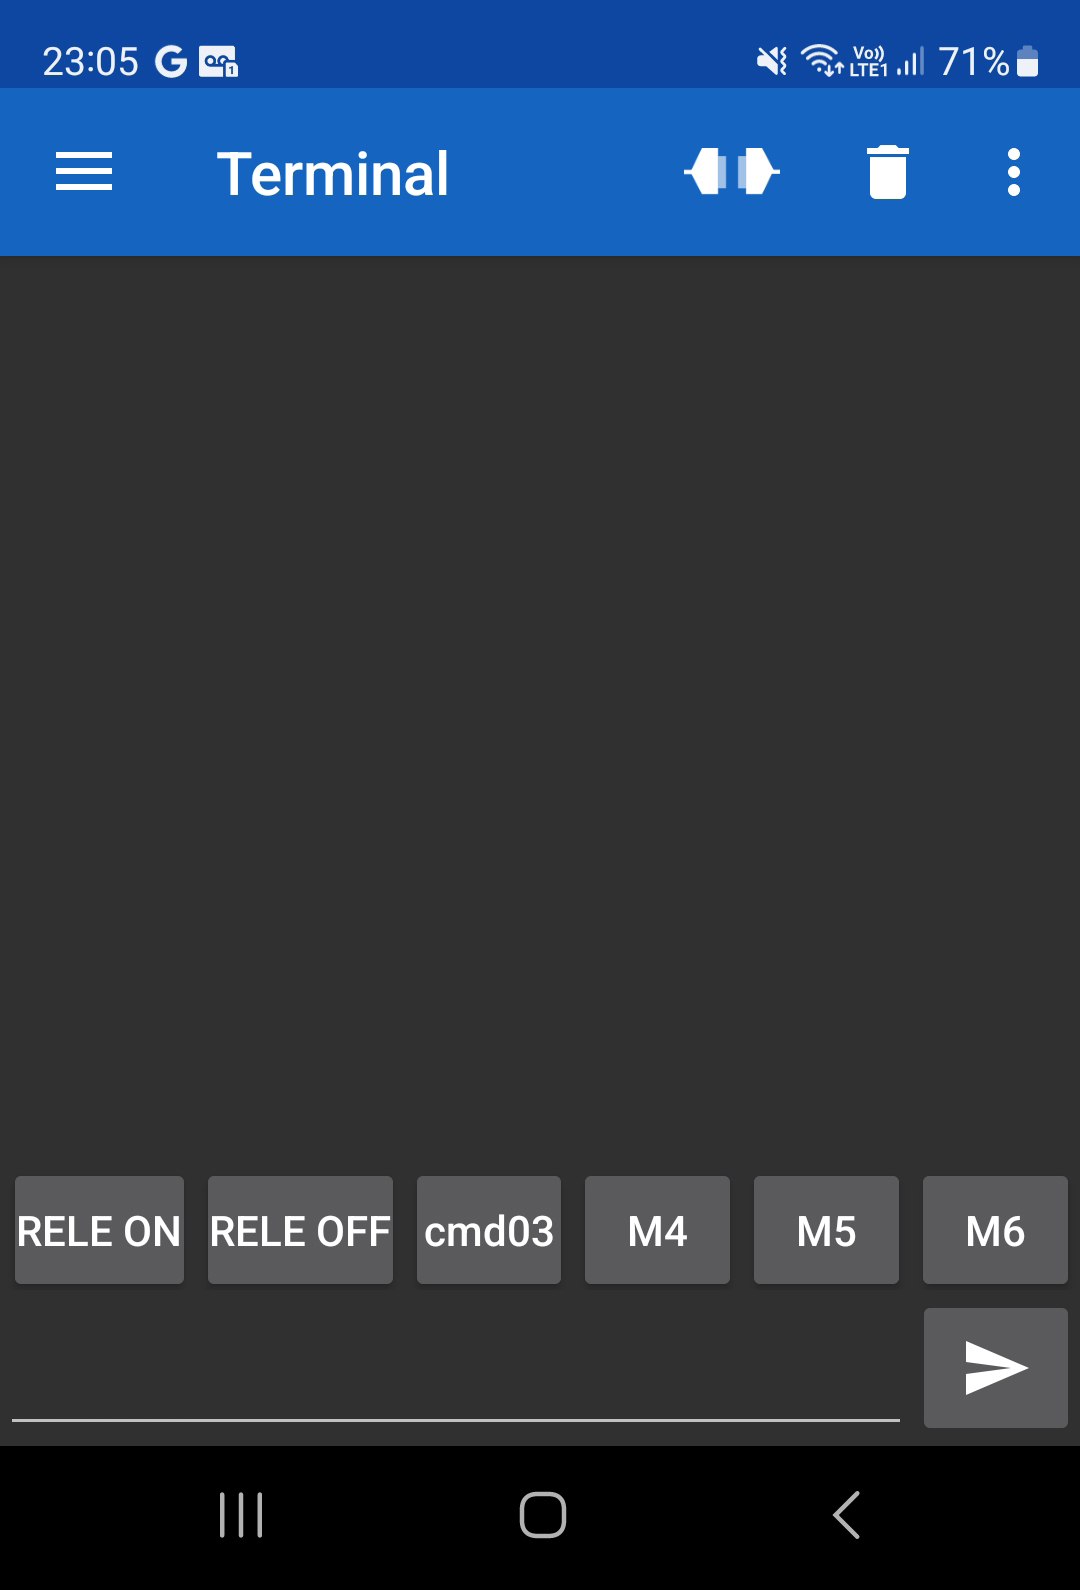
\includegraphics[width=0.40\textwidth]{figures/serialbluetoothterminal}
    \caption*{FONTE: Própria}
	\label{serialbluetoothterminal_tela}
\end{figure}
